% vim:ft=tex:
\documentclass[debug, font=Times]{gw-dissertation}[2021/11/19]
\usepackage{graphicx}
\usepackage{lipsum}  % to generate random paragraphs
\usepackage[none]{hyphenat}  % disable hyphenation; not required by GW guideline
\usepackage[style=numeric-comp]{biblatex}  % a modern alternative to bibtex
\sloppy  % to make long but non-hyphenated words go to the next line

% configuration for front pages (commands came from gw-dissertation class)
\title{Dissertation Title in Initial Capitals and Small Letters}
\author{Your Name}
\defdate{August 31, 2022}
\gradyear{2022}
\gradmonth{August}
\graddate{31}
\advisor{James W. Smith}{Professor of Finance}
\school{School of Engineering and Applied Science}
\dedication{\lipsum[4-5]}
\acknowledgments{\lipsum[4-5]}
\disclaimer{\lipsum[4-5]}
\abstract{\lipsum[4-5]}
\preface{\lipsum[4-5]}
\prevdegree{B.A. in Accounting, May 2006, University of Maryland}
\prevdegree{M.S. in Finance, January 2008, University of Maryland}
\committee{James W. Smith, Professor of Engineering, Dissertation Director}
\committee{Janet A. Doe, Associate Professor of Computer Science, University of Virginia, Committee Member}
\committee{Donald B. Green, Research Scientist, National, Committee Member}
\committee{Joseph Smith, Professor of History and of International Relations, Committee Member}
\committee{Joseph Smith, Associate Professor of History, University of Delaware, Committee Member}
\committee{Joseph Smith, Senior Researcher, American Historical Society, Committee Member}

% glossaries must be defined be in the preamble (or a tex file included in the preambel)
\newglossaryentry{ex}{name={sample},description={an example}}
\newabbreviation{svm}{SVM}{support vector machine}

% other configurations
\addbibresource{reference.bib}  % bib file location
\graphicspath{{figs}}  % default path to search for figures

% begin the dissertation
\begin{document}

\chapter{Introduction}

Start each chapter on a new page. All of the text on this page starts at the same location on the
ruler bar except for the first line of text of each new paragraph.

Note that each level is indented in a $1/4$ inch (or two dots to the right on the ruler bar) from
the last section header. 
    
    \section*{A dummy section header}
    This is a section without numbering. It is not going to present in ToC.

    \section{Second Level Header}
    \lipsum[6]

    \section{Second Level Header}
    \lipsum[4]

        \subsection{Third Level Header}
        \lipsum[5-6]

            \subsubsection{Fourth Level Header}
            Start your text here.

                \paragraph{Fifth Level Header}
                Start your text here.

\chapter{Literature Review or Your Heading}

Start your text and double-space the text.
\begin{figure}[h!]
    \centering
    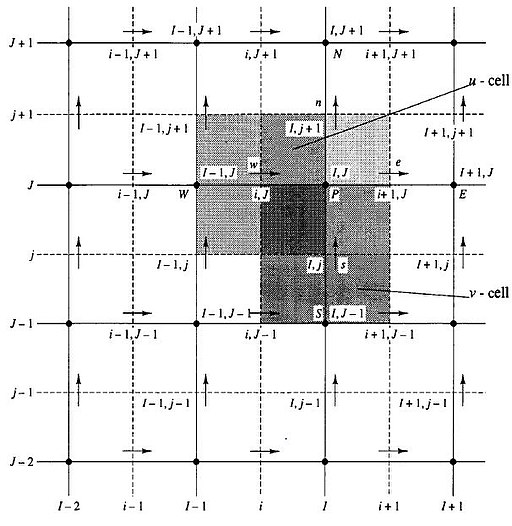
\includegraphics[width=0.5\linewidth]{grid.jpg}
    \caption{Staggered grid (public domain figure)}
\end{figure}
\begin{figure}[h!]
    \centering
    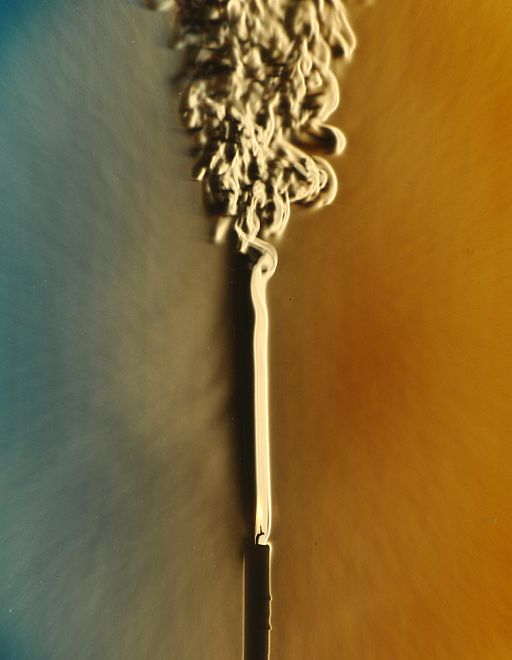
\includegraphics{laminar_turbulent_transition.jpg}
    \caption{%
        Laminar turbulent transition (public domain figure). I am trying to make the caption %
        longer so that we can see how this class handles long captions. I am trying to make the %
        caption longer so that we can see how this class handles long captions.%
    }
\end{figure}

\chapter{Methods or Your Heading}

Start your text and double-space the text.
\begin{figure}[h!]
    \centering
    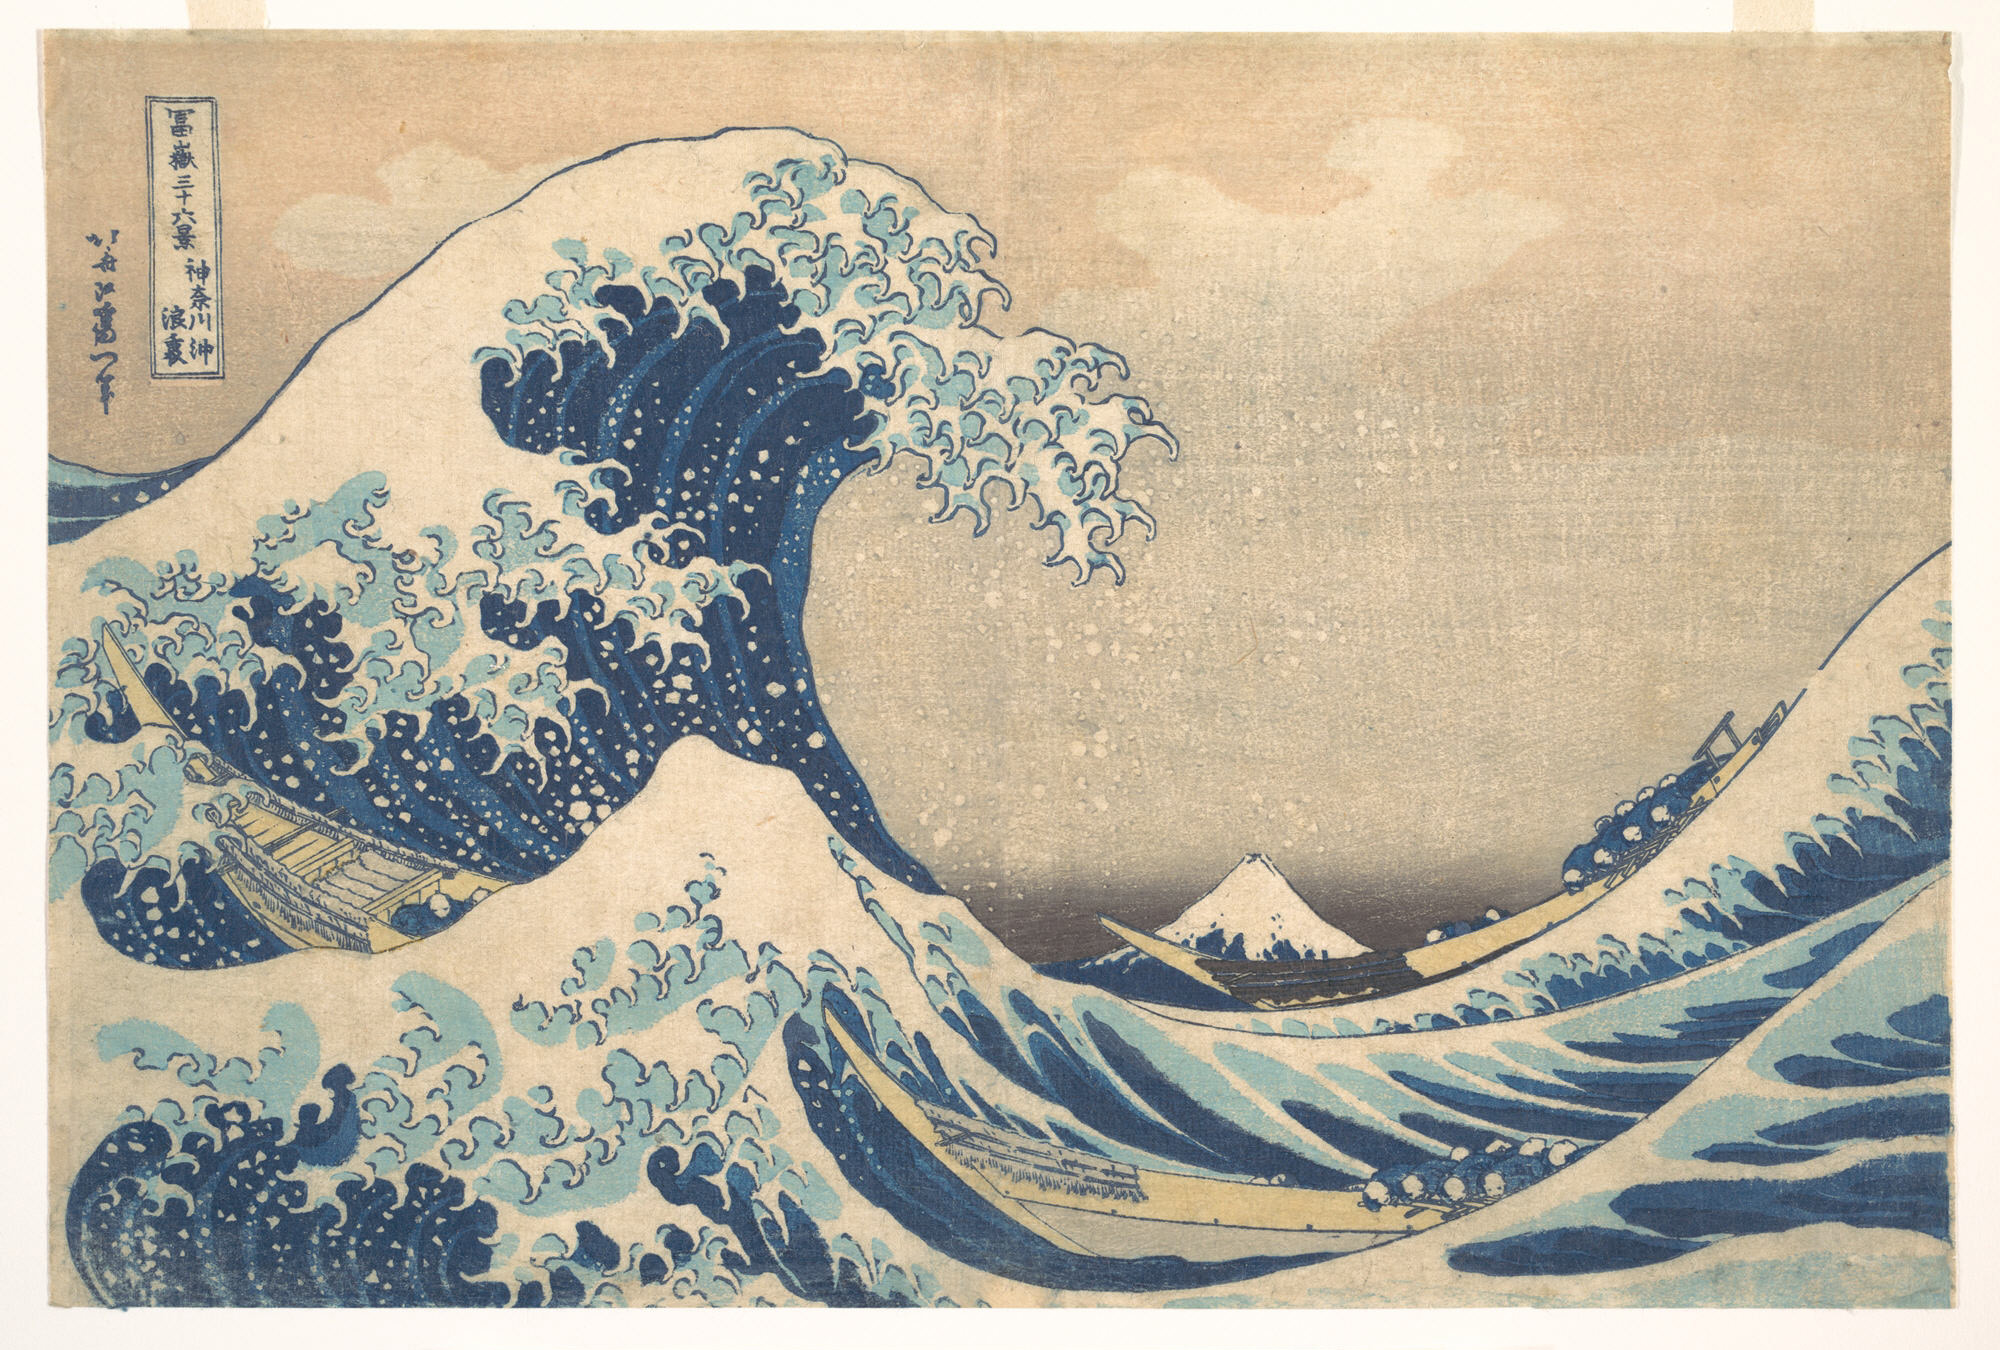
\includegraphics[width=0.5\linewidth]{the_great_wave.jpg}
    \caption{The Great Wave off Kanagawa by Katsushika Hokusai (public domain figure)}
\end{figure}

\chapter{Results or Your Heading}

Start your text and double-space the text.
\begin{table}[h!]
    \centering
    \begin{tabular}{||c c c c||}
         \hline
         Col1 & Col2 & Col2 & Col3 \\ [0.5ex]
         \hline\hline
         1 & 6 & 87837 & 787 \\
         2 & 7 & 78 & 5415 \\
         3 & 545 & 778 & 7507 \\
         4 & 545 & 18744 & 7560 \\
         5 & 88 & 788 & 6344 \\ [1ex]
         \hline
    \end{tabular}
    \caption{Example table 1}
\end{table}

\chapter{Discussion, Conclusion, or Your Heading}

Start your text and double-space the text. This is a fake citation \cite{author1_1990}. This is
another fake citation \cite{author2_2000}.
\begin{table}[h!]
    \centering
    \begin{tabular}{||c c c c||}
         \hline
         Col1 & Col2 & Col2 & Col3 \\ [0.5ex]
         \hline\hline
         1 & 6 & 87837 & 787 \\
         2 & 7 & 78 & 5415 \\
         3 & 545 & 778 & 7507 \\
         4 & 545 & 18744 & 7560 \\
         5 & 88 & 788 & 6344 \\ [1ex]
         \hline
    \end{tabular}
    \caption{Example table 2}
\end{table}

\sloppy
\printbibliography[heading=bibintoc, title=References]
\fussy

\appendix
\chapter{The Heading of Appendix A}

    \section{
        A very long section title is supposed to be rendered in single-line spacing within the entry
    }
    \lipsum[2]
    \begin{figure}[h!]
        \centering
        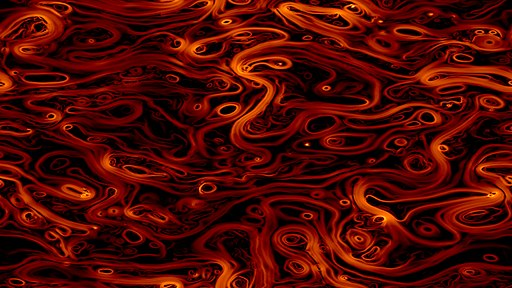
\includegraphics[width=0.5\linewidth]{magnetic_turbulence.jpg}
        \caption{Magnetic turbulence (public domain figure)}
    \end{figure}
    \lipsum[4]

        \subsection{Appendix Can Have Subsections}
        \lipsum[3]
        \begin{figure}[h!]
            \centering
            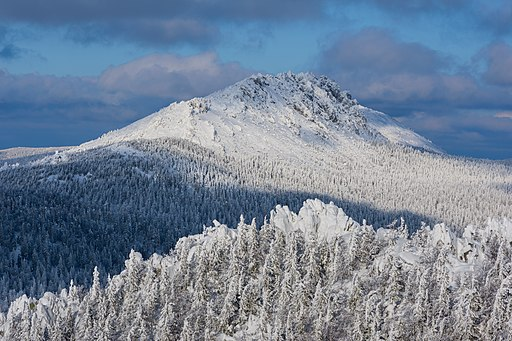
\includegraphics[width=0.5\linewidth]{mt_otkliknoy_greben.jpg}
            \caption{Mt. Otkliknoy Greben (public domain figure)}
        \end{figure}
        \lipsum[5]

        % on the contrary to glossaries, nomenclatures have to be in the document environment
        \nomenclature{$c$}{Speed of light in a vacuum}
        \nomenclature{$\alpha$}{
            A very long definition.  A very long definition.  A very long definition.
            A very long definition.  A very long definition.  A very long definition.
            A very long definition.  A very long definition.  A very long definition.
            A very long definition.  A very long definition.  A very long definition.
            A very long definition.
        }
        \nomenclature{$h$}{Planck constant}

    \section{Appendix Can Have Sections}
    \lipsum[6]

    Use \verb!\newglossaryentry! to define a glossary entry, and use \verb!\gls! to use it in the
    content.
    For example: \gls{ex}.

    Also, use \verb!\newabbreviation! to define abbreviations, and use \verb!\gls! to automatically show
    long and short expressions of this term based on the occurrence.
    For example first use: \gls{svm}, and second use: \gls{svm}.

    Terms in glossaries must be defined in the preamble.
    See the user manual of package \verb!glossaries!.

\chapter{
    The Heading of Appendix B
    The Heading of Appendix B
    The Heading of Appendix B
    The Heading of Appendix B
    The Heading of Appendix B
    The Heading of Appendix B
}
    \lipsum[7]
    \begin{table}[h!]
        \centering
        \begin{tabular}{||c c c c||}
             \hline
             Col1 & Col2 & Col2 & Col3 \\ [0.5ex]
             \hline\hline
             1 & 6 & 87837 & 787 \\
             2 & 7 & 78 & 5415 \\
             3 & 545 & 778 & 7507 \\
             4 & 545 & 18744 & 7560 \\
             5 & 88 & 788 & 6344 \\ [1ex]
             \hline
        \end{tabular}
        \caption{Example table 3}
    \end{table}
    \lipsum[1]

\end{document}
